\documentclass[11pt]{article}
\usepackage[utf8]{inputenc}
\usepackage[T1]{fontenc}
\usepackage{graphicx}
\usepackage[export]{adjustbox}
\graphicspath{ {./images/} }

\begin{document}
\section*{Reading}
Managing Long-Term Futures Exposures

Long positions in equities and real assets can typically be held indefinitely using a simple buy-and-hold strategy. However, futures and forward positions expire at settlement. To maintain a long-term exposure using futures or forward contracts, it is necessary to roll the positions over at or prior to their settlement dates. In other words, to maintain an exposure in the forward market, it is necessary to close a position in one contract as it approaches or reaches settlement and open a new position in a contract with the same underlying commodity but with a longer time to settlement. Rolling contracts refers to the process of closing positions in shortterm futures contracts and simultaneously replacing the exposure by establishing similar positions with longer terms. The rolling of contracts is an important part of maintaining long-term commodity exposures or hedges through futures and forward markets; this section provides foundational concepts on the issues involved.

\section*{Futures Contracts with Different Settlement Dates}
Futures contracts have regular settlement dates, as determined by the exchanges that created the contracts. A typical interval for settlement dates is quarterly, but especially among the shorter-term contracts, the interval can be monthly or even weekly. On an exchange, the futures contract with the shortest time to settlement is often referred to as the front month contract. The front month contract is sometimes referred to as the front contract, the nearby contract, or the spot contract. Contracts with longer times to settlement are often called distant contracts, deferred contracts, or back contracts. Deferred contracts are sometimes ranked as first deferred, second deferred, and so forth, denoting their order, with first deferred representing the deferred contract with the shortest time to settlement (after the front month) and so on.

The next exhibit illustrates the concept of regularly extending the settlement dates of the positions by closing nearby positions and opening deferred positions simultaneously to maintain a continuous exposure to the underlying commodity. The next exhibit simplifies the diagram by assuming that all of the opening trades occur at one price and that all of the closing trades occur at another price. In practice, the opening and closing prices would vary.

\begin{center}
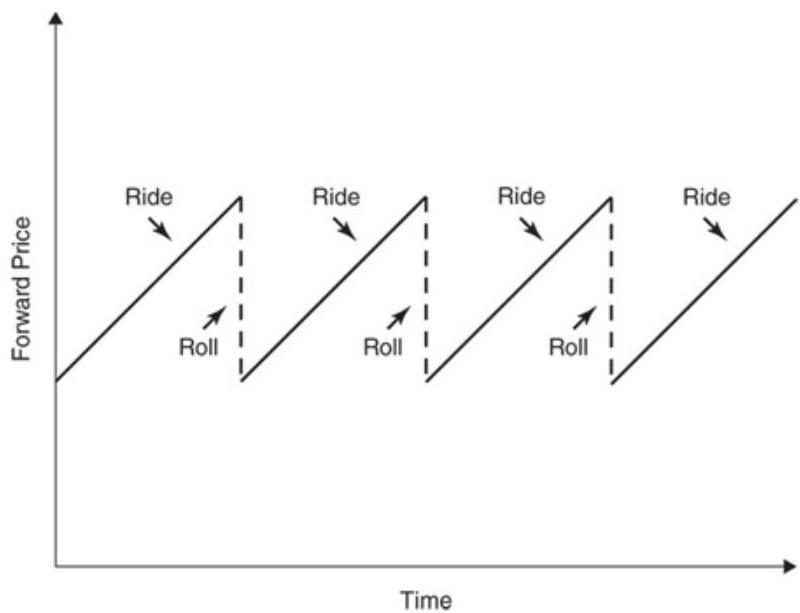
\includegraphics[max width=\textwidth]{2024_04_11_59506125c1e82061598cg-2}
\end{center}

\section*{Riding and Rolling of Forward and Futures Contracts}
To be consistent with concepts of finance other than commodities, the terminology for the process in the above exhibit would be that an investor holds, or rides, a given position as its time to settlement nears. At the point that the old position is closed and is replaced by a new position in the same commodity with a longer time to settlement, the investor is said to have rolled the position over. Thus, a long-term exposure can be constructed and maintained with a series of rides and rolls.

However, in commodities, the expression roll can also be used to describe the holding of a forward position through time.

\section*{Rollover Decisions Alter Long-Run Returns}
The timing of each rollover transaction is at the discretion of the investor. Some investors may wait until the contract settles or is about to settle before closing the old position and initiating a new position with a longer settlement date. Others may extend their settlement dates while their positions still have considerable time to settlement. Further, some investors may move into contracts with only a slightly longer time to settlement, whereas others may move into contracts with a much longer time to settlement.

The critical point is that, unlike financial assets such as equities, the long-term returns on futures contracts vary based on the particular decisions made by the holder of the position regarding the procedures used to extend the position into a longer position. The result is that the long-term returns of futures and forward contracts can be calculated only by making important assumptions about how and when the contracts are rolled over. Traders with different preferences for rolling contracts experience different long-term returns.


\end{document}